\documentclass[11pt]{scrartcl}
\usepackage{evan}

\theoremstyle{definition}
\newtheorem{axiom}{Axiom}
\renewcommand{\theaxiom}{\Roman{axiom}}
\ihead{Set Theory}
\ohead{Berkeley Math Circle}

\begin{document}
\title{BMC Intermediate II: Set Theory}
\date{January 13, 2015}
\maketitle

\begin{abstract}
  This is adapted from \url{https://blog.evanchen.cc/tag/set-theory/}.
  For more on set theory, you might see my course notes from Math 145: \url{https://evanchen.cc/coursework.html}.
\end{abstract}

\section{Setting Out}
For those of you that don't already know:
`$\forall$', `$\exists$' are shorthand for ``for all'' and ``exists'',
respectively.
`$\lor$' is short for ``or'' and `$\land$' is short for ``and''.
Also, `$\in$' means ``in''.

\begin{ques}
  What is a set?
\end{ques}
% {featherless bipeds} = {humans}
% Ask: what are some ways we can build sets

\begin{axiom}
  [Extensionality]
  \[ \forall A \forall B \forall x
    \left( x \in A \iff x \in B \right) \implies (A = B). \]
\end{axiom}

\begin{ques}
  [Russell's Paradox]
  Define $X = \left\{ \text{sets $S$} \mid S \notin S \right\}$.
  Does $X$ contain itself?
\end{ques}

% explain here: we write down axioms using our intuition,
% but then any disagreement about what a set is we refer to the axioms

\section{Constructive ZF Axioms}
\begin{ques}
  What are some ways to build sets?
\end{ques}
% Ask: who can tell me some ways to build sets?

\begin{axiom}
  [Empty Set Exists] $\exists \varnothing : \forall x \; (x \notin \varnothing)$.
\end{axiom}
% Ask: Why is this set unique?

\begin{axiom}
  [Pairing] $ \forall x \forall y \exists A: \quad \forall z, \; z \in A \iff \left( (z=x) \lor (z=y) \right). $
\end{axiom}
% Ask: Why is this set unique?

\begin{axiom}
  [Union] $ \forall a \exists z \quad \forall x \; (x \in z) \iff (\exists y : x \in y \in z) $
\end{axiom}
% Ask: Why is this unique?

\begin{axiom}
  [Replacement]
  Let $f$ be a function on a set $X$ defined by a formula in LST.
  Then the image of $f$ is a function:
  \[ \exists Y : \quad \forall y, \; y \in Y \iff \exists x : f(x) = y. \]
\end{axiom}
\begin{axiom}
  [Restricted Comprehension]
  Let $\phi$ be some property, and let $S$ be a set.
  Then $ \left\{ x \in S \mid \phi(x) \right\} $
  is a set.
\end{axiom}
(Actually, Comprehension follows from Replacement.)

\begin{axiom}
  [Power Set] We can construct the power set $\mathcal P(X)$. Formally,
  \[ \forall X \exists A: \quad \forall Y (Y \in A \iff Y \subseteq X) \]
  where $Y \subseteq X$ is short for $\forall z (z \in Y \implies z \in X)$.
\end{axiom}

\section{The von Neumann Universe}
\[
  V_0 = \varnothing \qquad
  V_{n+1} = \mathcal P(V_n) \qquad
  V_{\lambda} = \bigcup_{\alpha < \lambda} V_\alpha
\]
\begin{center}
  \begin{asy}
    size(9cm);
    pair A = (10,30);
    pair B = -conj(A);
    pair O = origin;
    MP("V", A, dir(10));
    draw(O--A--B--cycle);
    MP("V_0 = \varnothing", O, dir(-20));
    draw(MP("V_\omega = \bigcup V_n", 0.7*A, dir(0))--0.7*B);
    draw(MP("V_{n+1} = \mathcal P(V_n)", 0.45*A, dir(0))--0.45*B);
    draw(MP("V_n", 0.4*A, dir(0))--0.4*B);
    MP("V_1 = \{\varnothing\}", 0.05*A, dir(0));
    MP("V_2 = \{\varnothing, \{\varnothing\} \}", 0.10*A, dir(0));
    draw(O--MP("\text{On}", midpoint(A--B), dir(90)));
  \end{asy}
\end{center}

\section{Foundation}
\begin{axiom}
  [Foundation] The relation $\in$ is well-founded,
  meaning there are no infinite descending $\in$-chains:
  \[ y_0 \ni y_1 \ni y_2 \ni y_3 \ni \dots. \]
\end{axiom}
\begin{ques}
  Why can no set contain itself?
\end{ques}


%\section{Well-Founded Relations}
%Let $\prec$ be a relation.
%\begin{itemize}
%  \ii a \emph{total ordering} if any two elements can be compared, strict and transitive,
%  \ii \emph{well-founded} if any set has a $\prec$-minimal element,
%  \ii a \emph{well-ordering} if both above conditions hold.
%\end{itemize}
%\begin{itemize}
%  \ii $\sim$ is an \emph{equivalence relation} if it is reflexive, symmetric, and transitive.
%  \ii $\sim$ is a \emph{partial ordering} if it is anti-reflexive and transitive.
%  \ii $\sim$ is a \emph{total ordering} if it is a partial ordering and any two elements are related.
%  \ii $\sim$ is \emph{well-founded} if it is a partial ordering with the property that any nonempty subset of $X$ has a minimal element.
%  \ii $\sim$ is an \emph{well-ordering} if it is a well-founded total ordering.
%\end{itemize}

\section{Encoding}
\begin{itemize}
  \ii $(x,y) \defeq \left\{ \left\{ x \right\}, \left\{ x,y \right\} \right\}$.
  \ii $\sim \defeq \left\{ (x,y) \mid x \sim y \text{ and } x,y \in X \right\}$.
  \ii $f \defeq \left\{ (x, f(x)) \mid x \in X \right\}$.
  \ii $0 \defeq \varnothing$ and $5 \defeq \left\{ 0, 1, 2, 3, 4 \right\}$.
\end{itemize}

\section{Ordinals}
A set is \emph{transitive} if $\in$ is transitive on it.
We define an \emph{ordinal} to be a transitive set which is \emph{well-ordered} by $\in$.

\begin{axiom}
  [Infinity] There exists a set
  $\omega = \left\{ 0,1,2,3,\dots \right\}$.
\end{axiom}

\begin{center}
  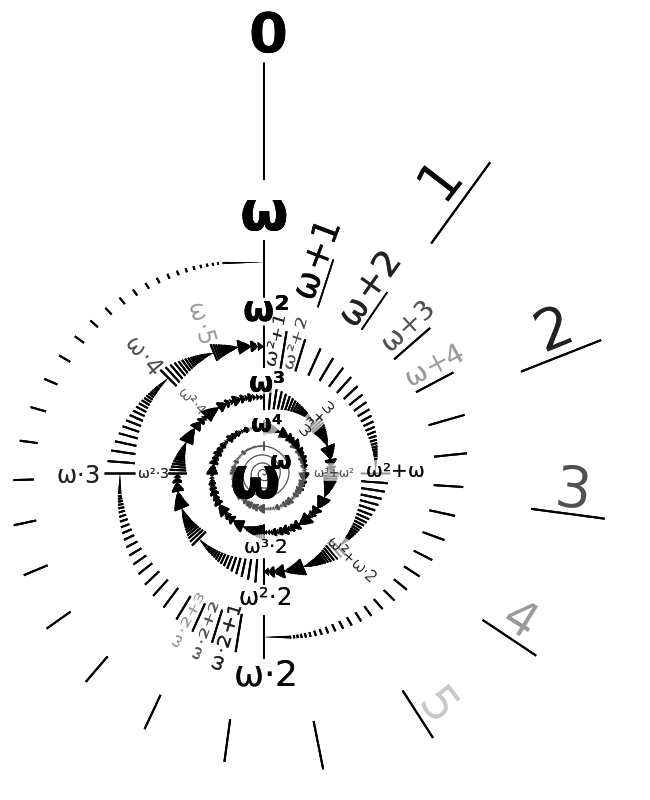
\includegraphics[width=7cm]{ordinal-spiral.png}

  { \scriptsize Public domain: \url{http://commons.wikimedia.org/wiki/File:Omega-exp-omega-labeled.svg} }
\end{center}

Note that there are no descending $\in$ chains.
We can also distinguish between \emph{successor ordinals} and \emph{limit ordinals}.
You can even induct on these ordinals.

\begin{remark*}
  Note that all the above ordinals are actually countable.
  In particular, there are bijections between all the infinite ordinals in the above spiral.
  Thus ordinals are not a great way of keeping track of ``sizes''.
  The way to fix this is to define a \emph{cardinal} as an ordinal
  which is not in bijection with any smaller ordinal.
\end{remark*}

\begin{ques}
  Why do all sets appear in some $V_\alpha$?
\end{ques}

\section{Ordinal Arithmetic}
Addition:
\[ \alpha + \beta
  \defeq
  \opname{ot}\left(
  \left( \{0\} \times \alpha \right) \cup \left( \{1\} \times \beta \right),
  <_{\text{lex}}
  \right). \]
Alternatively, by transfinite induction,
\begin{align*}
  \alpha + 0 &= \alpha \\
  \alpha + (\beta + 1) &= (\alpha + \beta) + 1 \\
  \alpha + \lambda &= \bigcup_{\beta < \lambda} (\alpha + \beta).
\end{align*}
Multiplication:
\[ \alpha \cdot \beta
  =
  \opname{ot}\left( \beta \times \alpha, <_{\text{lex}} \right). \]
Alternatively, by transfinite induction,
\begin{align*}
  \alpha \cdot 0 &= \alpha \\
  \alpha \cdot (\beta + 1) &= (\alpha \cdot \beta) + \alpha \\
  \alpha \cdot \lambda &= \bigcup_{\beta < \lambda} \alpha \cdot \beta.
\end{align*}

\section{Cardinals}
A \emph{cardinal} is an ordinal $\kappa$ which is not in bijection
with any lesser ordinal.
They can also be indexed by ordinals:
\[ \aleph_0, \aleph_1, \aleph_2, \dots, \aleph_{\omega}, \aleph_{\omega+1}, \dots \]

\begin{itemize}
  \ii Cantor's diagonal argument states that $2^\kappa > \kappa$.
  \ii Continuum Hypothesis: $2^{\aleph_0} = \aleph_1$.
\end{itemize}

\section{The Axiom of Choice}
\begin{axiom}
  [Choice] Given a set $Y$ of nonempty sets, one can construction a \emph{choice} function $f : Y \to \mathcal P(Y)$ such that $f(X) \in X$ for every $X \in Y$.
\end{axiom}
\begin{problem*}
  There are infinitely many people in a room, each wearing or red, green, or blue hat.
  At a signal, everyone simultaneously tries to guess the color of his or her hat.
  Prove that they can devise a strategy such that at most finitely many people
  guess incorrectly.
\end{problem*}

% AC, ordinal arithmetic
% AC <=> WO
% Hats problem
% transfinite induction and recursion!
% cardinals

\end{document}
